\section{Applications of convolution - Filters ( Image processing )}
\subsection{Gaussian filter}
\begin{enumerate}
\item A Gaussian filter is a type of digital filter that utilizes a Gaussian distribution function to smooth and reduce noise in signals or images. It achieves this by averaging neighboring values with weights based on a Gaussian curve, giving more weight to the central value and less to the outer values.
\item One dimensional Gaussian - \\
\begin{align}
	G_{1} (x) &= \frac{1}{\sqrt{2 \pi \sigma^2}} e^{-\frac{x^2}{2 \sigma^2}}
\end{align} \\
Two-dimensional Gaussian - \\
\begin{align}
	G_{2} (x) &= \frac{1}{\sqrt{2 \pi \sigma^2}} e^{-\frac{x^2 + y^2}{2 \sigma^2}}
\end{align} \\
\item \textbf{How it works ?} 
\begin{itemize}
\item A Gaussian filter, is a low-pass filter, that uses a kernel that represents the weighting of neighboring pixels. 
\item The kernel is then convolved with the image ( i.e., it is moved across the image ), and the values of the kernel are multiplied by the corresponding pixel values in the image. 
\item The products are then summed, and the result is divided by the sum of the kernel values, producing a weighted average of the pixel's neighborhood. 
\item The weighted average becomes the new value of the pixel at the center of the kernel's position, smoothing out the image.
\end{itemize}
\item The corresponding figure is shown below - \\
\begin{figure}[h]
    \centering
    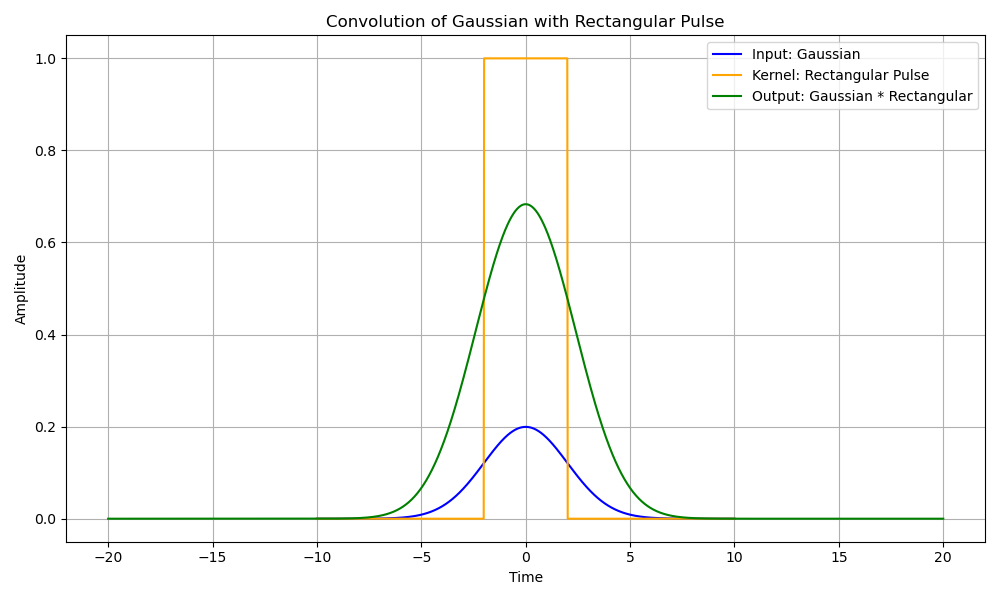
\includegraphics[width=0.6\textwidth]{figs/gaus_2.png}
    \caption{T = 2}
    \label{fig:gaus_2}
\end{figure}
\begin{figure}[h]
    \centering
    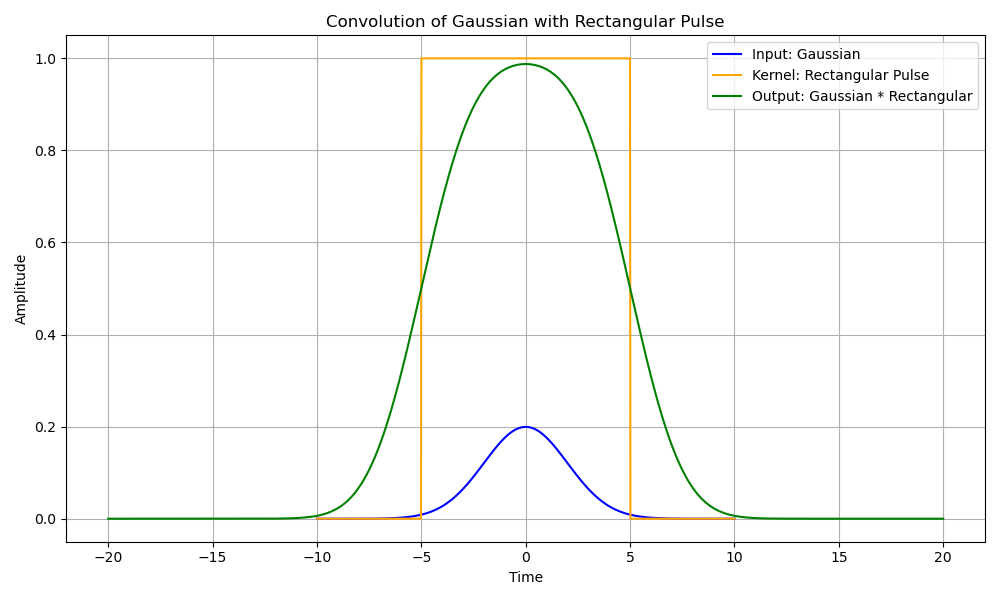
\includegraphics[width=0.6\textwidth]{figs/gaus_5.png}
    \caption{T = 5}
    \label{fig:gaus_0.5}
\end{figure}
\begin{figure}[h]
    \centering
    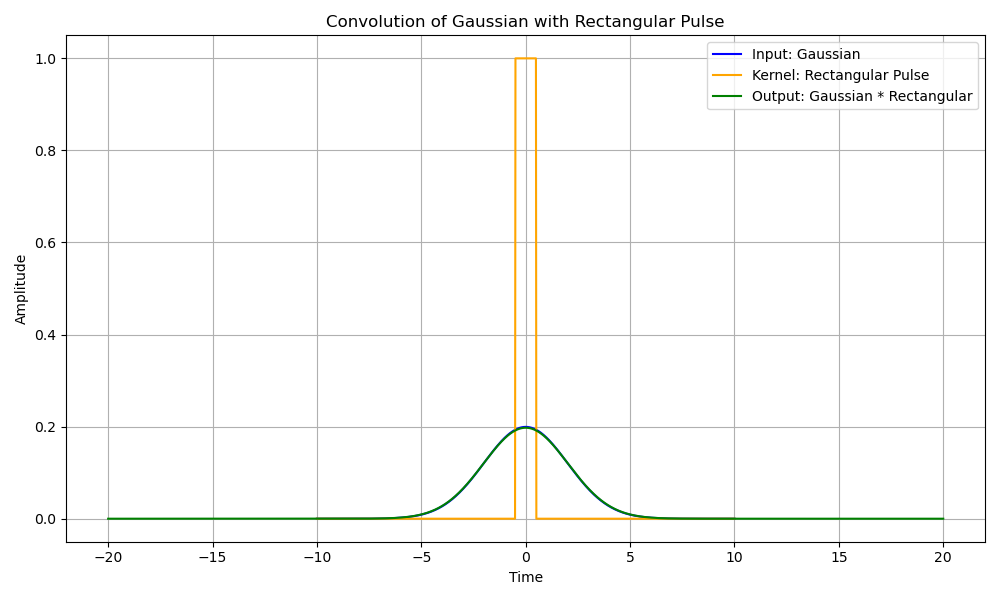
\includegraphics[width=0.6\textwidth]{figs/gaus_0.5.png}
    \caption{T = 0.5}
    \label{fig:gaus_0.5}
\end{figure}

\item In the case of Figure \ref{fig:gaus_0.5}, since the kernel itself is bell-shaped, convolving a narrow Gaussian will produce an output being very similar to the original signal, just slightly smoothed or blurred.
\item Gaussian filters are used because - \\
\begin{itemize}
\item Smooth
\item Decay to zero rapidly
\item Simple analytical formula
\item \textbf{Central Limit Theorem :} Limit of applying filters many times is some Gaussian.
\item Separable
\begin{align*}
	G_{2} (x, y) &= G_{1} (x) G_{1} (y)
\end{align*}
\end{itemize}
\end{enumerate}

\subsection{Laplacian filter}
\begin{enumerate}
\item A Laplacian filter is a second-order derivative operator that is commonly used in image processing for edge detection and enhancement.
\item It is often implemented using a convolution kernel, which is a small matrix that is slid over the image and multiplied with the surrounding pixels to produce a new pixel value.
\item The Laplacian filter, when combined with a Gaussian blur ( Laplacian of Gaussian ), can be used to detect edges in an image.
\item Image corresponding to this is given below - \\
\begin{figure}[h]
    \centering
    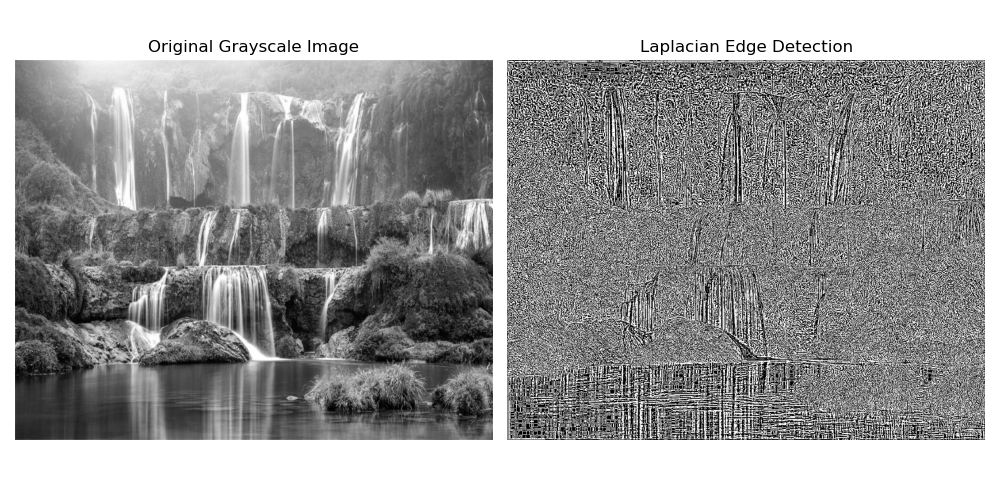
\includegraphics[width=0.6\textwidth]{figs/laplace.png}
    \caption{Edge detection using convolution}
    \label{fig:laplace}
\end{figure}
\end{enumerate}
